\documentclass[serif,xcolor=pdftex,dvipsnames,table,hyperref={bookmarks=false}]{beamer}

%%%%%%%%%%%%%%%%
% Change the macros below to configure the title slides
% for your course.
\newcommand{\coursename}{COMPSCI 589}
\newcommand{\instructor}{Benjamin M. Marlin}
\newcommand{\university}{University of Massachusetts Amherst}
\newcommand{\department}{College of Information and Computer Sciences}
%%%%%%%%%%%%%%%%


\newcommand{\settitlecard}[2]{
  \title[\coursename  Lecture #1] 
    {\coursename \\ Lecture #1: #2}
     \author[\instructor]{\instructor}
     \institute[\university]{
     \department\\
     \university
   }
\date{}
}

\newcommand{\maketitlepage}{
  \begin{frame}
  \titlepage
  \center{
    %If you use the slides unmodified, retain the attribution below
    \tiny{Slides by Benjamin M. Marlin (marlin@cs.umass.edu). \\
    \vspace{-1em}Created with support from National Science Foundation Award\# IIS-1350522. 
    %If you modify the slides, please retain the alternate attribution below
    %\tiny{Based on slides by Benjamin M. Marlin (marlin@cs.umass.edu). \\    
    %\vspace{-1em}Created with support from National Science Foundation Award\# IIS-1350522. 
    }                                              
  }  
  \end{frame}
}

\AtBeginSection[]
{
  \begin{frame}<beamer>{Outline}
    \tableofcontents[currentsection,subsectionstyle=hide]
  \end{frame}
}


\newcommand{\cut}[1]{}

\newcommand{\iconbox}[4]{
  \only<#1-#2>{
    \begin{columns}[T]
      \column{0.5in}
           \includegraphics[width=0.5in]{#3}
       \column{3.7in}
            #4
    \end{columns}
    \medskip
    \medskip
    \medskip
  }
}

\mode<presentation>{
  \usepackage{../beamertheme589theme}
  \setbeamercovered{invisible}
}

\mode<handout>{
  \usepackage{../beamertheme589theme}
  \setbeamercovered{transparent}
}


\usepackage[english]{babel}
\usepackage[latin1]{inputenc}
\usepackage{times}
\usepackage[T1]{fontenc}
\usepackage{amsmath}
\usepackage{amssymb}
\usepackage[noend]{algorithmic}
\usepackage{algorithm}
\usepackage{listings}

\renewcommand\mathfamilydefault{\rmdefault}

\newcommand{\setA}{\mathcal{A}}
\newcommand{\setB}{\mathcal{B}}
\newcommand{\setS}{\mathcal{S}}
\newcommand{\setV}{\mathcal{V}}
\DeclareMathOperator*{\union}{\bigcup}
\DeclareMathOperator*{\intersection}{\bigcap}
\DeclareMathOperator*{\Val}{Val}
\newcommand{\mbf}[1]{{\mathbf{#1}}}
\DeclareMathOperator*{\argmax}{arg\,max}
\DeclareMathOperator*{\argmin}{arg\,min}
\DeclareMathOperator*{\sign}{sign}
\newcommand{\deriv}[2]{\frac{\partial{#1}}{\partial{#2}}}


\settitlecard{4}{Overfitting, Regularization,\\ and Crossvalidation}

\begin{document}

\maketitlepage

\section{Review}
\subsection{Foo}

\begin{frame}[t]{Open Questions}

\begin{itemize}
\setlength{\itemsep}{8pt}
\item To date we have introduced five classifiers: KNN, Decision Trees, Naive Bayes, LDA and Logistic Regression.

\pause\item In the case of KNN and Decision Trees, we saw that the results are very sensitive to the number of neighbors, and the depth of the tree. 

\pause\item In the case of logistic regression, we saw that $P_{\mbf{w}}(y|\mbf{x})$ is 
sensitive to the magnitude of the weights $\mbf{w}$. 

\pause\item In this lecture, we'll discuss what changes in these models as we vary these parameters and introduce methodology for selecting optimal values for them.

\end{itemize}

\end{frame}


\section{Capacity and Generalization}
\subsection{Foo}


\begin{frame}[t]{Model Capacity}

\begin{itemize}
\setlength{\itemsep}{12pt}

\item Deterministic classifiers that can represent more complex decision boundaries are said to have higher \textit{capacity} than classifiers that can only represent simpler boundaries. 

\pause\item Probabilistic classifiers that can represent more complex sets of conditionals $P(Y|X)$
are said to have higher \textit{capacity} than probabilistic classifiers that can only represent simpler sets of conditionals. 

\pause\item \textbf{Question:} How would you rank the capacity of the classifiers we've seen so far?

\end{itemize}

\end{frame}

\begin{frame}[t]{Generalization}

\begin{itemize}
\setlength{\itemsep}{12pt}

\item \textbf{Question:} Why can't we always just use the classifier with the highest possible capacity for every problem? 

\pause\item \textbf{Answer:} This would always minimize the error on the training data. However, what we really care about for prediction problems is \textit{generalization}.

\pause\item \textbf{Generalization:} The ability of a trained classifier to achieve an error rate on \textit{future, unseen examples} (the generalization error rate) that is comparable to the training error rate. 

\pause\item \textbf{Capacity Control:} To achieve optimal generalization performance for a given training set, we often need to control model capacity carefully. 

\end{itemize}

\end{frame}

\begin{frame}[t]{Overfitting and Underfitting}

\begin{itemize}
\setlength{\itemsep}{12pt}

\item \textbf{Overfitting:} The generalization error for a classifier is much worse than the training error. This usually results from choosing a classifier with too much capacity so that it models the noise in the training data.

\item \textbf{Underfitting:} Occurs when the capacity of the classifier is too low to capture the actual structure in the training data, leading to both high training error and high generalization error.

\end{itemize}

\end{frame}


\begin{frame}[t]{Bias-Variance Trade-Off}

\begin{itemize}
\setlength{\itemsep}{12pt}

\item \textbf{Bias:} A classifier is said to have low \textit{bias} if the true decision boundary or conditionals $P(Y|X)$ can be approximated closely by the model.

\pause\item \textbf{Variance:} A classifier is said to have low \textit{variance} if the decision boundary or conditionals $P(Y|X)$ it constructs are stable with respect to small changes to the training data. 

\pause\item \textbf{Bias-Variance Dilemma:} To achieve low generalization error, we need classifiers that are low-bias and low-variance, but this isn't always possible. 

\pause\item \textbf{Bias-Variance and Capacity:} On complex data, models with low capacity have low variance, but high bias; while models with high capacity have low bias, but high variance. 
\end{itemize}
\end{frame}

\section{Hyperparameters}
\subsection{foo}

\begin{frame}[t]{Hyperparameters}

\begin{itemize}
\setlength{\itemsep}{12pt}

\item In order to control the capacity of a classifier, it needs to have capacity control parameters. 

\pause\item Because capacity control parameters can not be chosen based on training error, they are often called hyperparameters. 

\pause\item \textbf{Question:} What are the capacity control parameters for KNN and decision trees?

\pause\item \textbf{Question:} What are the capacity control parameters for naive Bayes and logistic regression? 

\end{itemize}
\end{frame}

\begin{frame}[t]{Capacity, Smoothness and Regularization}

\begin{itemize}
\setlength{\itemsep}{6pt}

\item \textbf{Capacity and Smoothness:} In the case of probabilistic classifiers like NB, LDA, and LR, we can think of capacity in terms of the \textit{smoothness} of $P(Y|X)$. 

\pause\item \textbf{Regularization:} We can control the smoothness of $P(Y|X)$ using a technique called \textit{regularization} that penalizes parameters that result in overly complex $P(Y|X)$ during learning.

\pause\item \textbf{Laplace Smoothing:} Laplace smoothing is a simple method for smoothing the parameter estimates of a categorical distribution:

$$P_{\theta}(X=v)=\theta_v = \frac{\alpha + \sum_{i=1}^n[x_i=v]}{V\alpha + n}, \;\; v=1..V$$

\pause\item As the regularization hyperparameter $\alpha$ increases, our estimate of the distribution smooths out toward being uniform. This provides capacity control for NB with binary or categorical features. 


\end{itemize}
\end{frame}

\begin{frame}[t]{Regularization For Logistic Regression}

\begin{itemize}
\setlength{\itemsep}{6pt}

\item In the case of logistic regression, the smoothness of $P_{\mbf{w}}(Y|X)$ is determined by the magnitude of $\mbf{w}$. 

\pause\item We can control the magnitude of $\mbf{w}$ by introducing a regularization term into the conditional log likelihood learning criteria that penalizes the norm of $\mbf{w}$. 

\pause
$$\theta_* = \argmax_{\theta}\;\;\sum_{i=1}^n \log P(Y=y_i|\mbf{X}=\mbf{x}_i) - \lambda ||\mbf{w}||_2^2 $$

\pause\item Some formulations of this problem up-weight the contribution from the data instead:

$$\theta_* =  \argmax_{\theta}\;\; C\sum_{i=1}^n \log P(Y=y_i|\mbf{X}=\mbf{x}_i) - ||\mbf{w}||_2^2 $$

\end{itemize}
\end{frame}

\begin{frame}[t]{Regularization For Logistic Regression}

\begin{itemize}
\setlength{\itemsep}{6pt}

\item This problem can also be solved using other norms, including the $\ell_1$ norm. This has the advantage of creating sparse weight vectors: 

\pause
$$\theta_* =  \argmax_{\theta}\;\;\sum_{i=1}^n \log P(Y=y_i|\mbf{X}=\mbf{x}_i) - \lambda ||\mbf{w}||_1 $$

$$\theta_* = \argmax_{\theta}\;\; C\sum_{i=1}^n \log P(Y=y_i|\mbf{X}=\mbf{x}_i) - ||\mbf{w}||_1 $$

\pause\item The regularization hyperparameters are either $\lambda$ or $C$. As $\lambda$ increases, the learned $P(Y|X)$ will smooth out. As $C$ decreases, the learned $P(Y|X)$ will smooth out.

\end{itemize}
\end{frame}

\section{Model Selection and Evaluation}
\subsection{foo}

\begin{frame}[t]{Model Selection and Evaluation}
\begin{itemize}
\setlength{\itemsep}{12pt}

\item We've identified the parameters that control the capacity of our models, we need a way to choose optimal values for these parameters. 

\pause\item In addition, we will want an estimate of the generalization error that the selected parameters achieve.

\pause\item To obtain, valid results, we need to use appropriate methodology and construct learning experiments carefully.

\pause\item\textbf{Guiding Principle:} Data used to estimate generalization error can not be used for any other purpose (ie: model training, hyperparameter selection, feature selection, etc.) or the results of the evaluation will be \textbf{biased}.

\end{itemize}
\end{frame}


\begin{frame}[t]{Recipe 1: Train-Validation-Test}
\begin{itemize}
\setlength{\itemsep}{6pt}

\item Given a data set $D$, we randomly partition the data cases into a training set ($Tr$), a validation set ($V$), and a test set ($Te$). Typical splits are 60/20/20, 80/10/10, etc. 

\pause\item Models $M_i$ are learned on $Tr$ for each choice of hyperparameters $H_i$

\pause\item The validation error $Val_i$ of each model $M_i$ is evaluated on $V$.

\pause\item The hyperparameters $H_*$ with the lowest value of $Val_i$ are selected and the classifier is re-trained using these hyperparameters on $Tr+V$, yielding a final model $M_*$

\pause\item Generalization performance is estimated by evaluating error/accuracy of $M_*$ on the test data $Te$.

\end{itemize}
\end{frame}


\begin{frame}[t]{Example: Train-Validation-Test}

\center
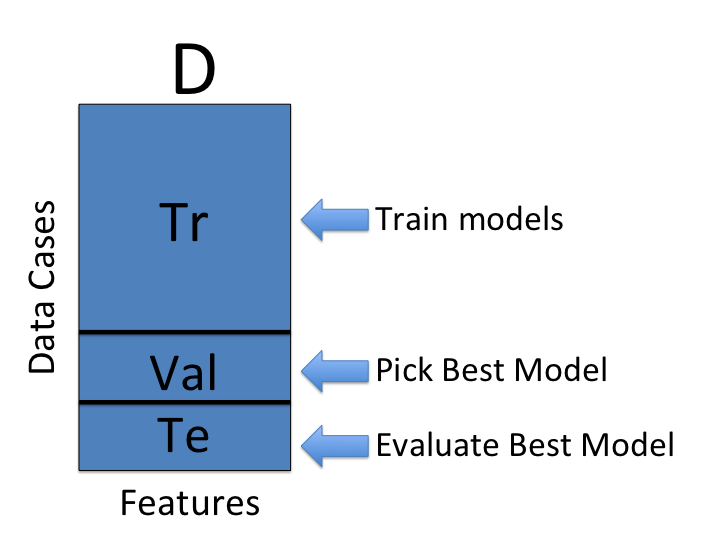
\includegraphics[width=2.8in]{../Figures/model-selection-tr-val-te.png}

Note that the order of the data cases needs to be randomly
shuffled before partitioning D.

\end{frame}


\begin{frame}[t]{Recipe 2: Crossvalidation-Test}
\begin{itemize}
\setlength{\itemsep}{6pt}

\item Randomly partition $D$ into a learning set $L$ and a test set $Te$ (typically 50/50, 80/20,  etc). 

\pause\item We next randomly partition $L$ into a set of $K$ blocks $B_1,...,B_K$.

\pause \item For each crossvalidation fold $k=1,...,K$:
\begin{itemize}
  \pause\item Let $V=B_k$ and $Tr = L/B_k$ (the remaining  $K-1$ blocks).
  \pause\item Learn $M_{ik}$ on $Tr$ for each choice of hyperparameters $H_i$.
  \pause\item Compute $Val_{ik}$ of $M_{ik}$ on $V$.
\end{itemize}
\pause\item Select hyperparameters $H_*$ minimizing $\frac{1}{K}\sum_{k=1}^K Val_{ik}$ and re-train model on $L$ using these hyperparameters, yielding final model $M_*$.

\pause\item Estimate generalization performance by evaluating error/accuracy of $M_*$ on $Te$.

\end{itemize}

\end{frame}

\begin{frame}[t]{Example: 3-Fold Cross Validation and Test}
\center
First Cross Validation Fold\\
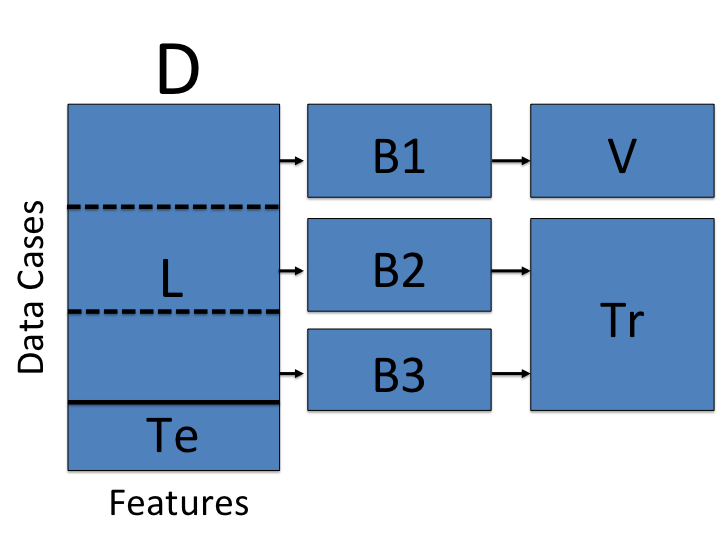
\includegraphics[width=2.8in]{../Figures/model-selection-cv-te-1.png}\\
Note that the order of the data cases needs to be randomly
shuffled before partitioning D into L and Te. 
\end{frame}

\begin{frame}[t]{Example: 3-Fold Cross Validation and Test}
\center
Second Cross Validation Fold\\
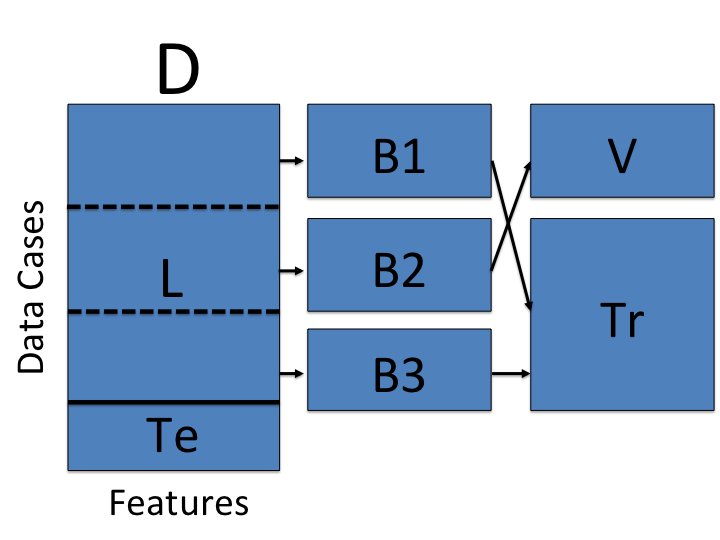
\includegraphics[width=2.8in]{../Figures/model-selection-cv-te-2.png}\\
Note that the order of the data cases needs to be randomly
shuffled before partitioning D into L and Te.  
\end{frame}

\begin{frame}[t]{Example: 3-Fold Cross Validation and Test}
\center
Third Cross Validation Fold\\
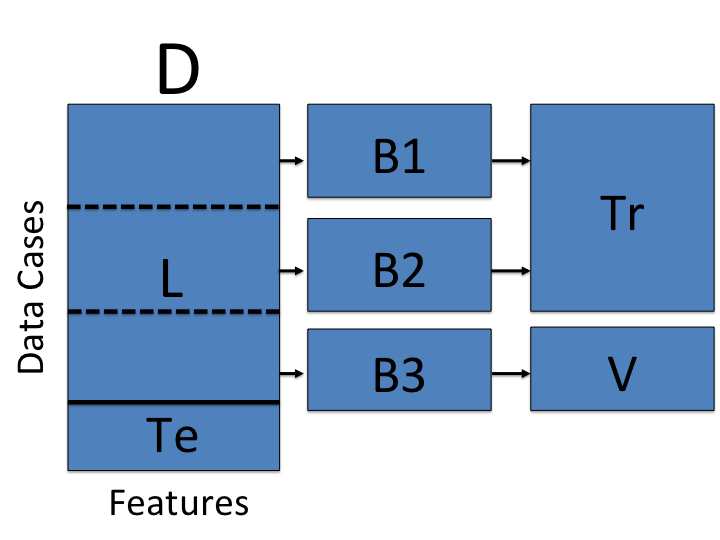
\includegraphics[width=2.8in]{../Figures/model-selection-cv-te-3.png}\\
Note that the order of the data cases needs to be randomly
shuffled before partitioning D into L and Te. 
\end{frame}


\begin{frame}[t]{Recipe 3: Random Resampling Validation-Test}
\begin{itemize}
\setlength{\itemsep}{6pt}

\item Randomly partition the data cases into a learning set $L$ and a test set $Te$ (typically 50/50, 80/20,  etc). 

\pause \item For sample $s=1,...,S$:
\begin{itemize}
  \pause\item Randomly partition $L$ into $Tr$ and $V$ (again 50/50, 80/20, etc).
  \pause\item Learn $M_{is}$ on $Tr$ for each choice of hyperparameters $H_i$.
  \pause\item Compute $Val_{is}$ of $M_{is}$ on $V$.
\end{itemize}
\pause\item Select hyperparameters $H_*$ minimizing $\frac{1}{S}\sum_{s=1}^S Val_{is}$ and re-train model on $L$ using these hyperparameters, yielding final model $M_*$.

\pause\item Estimate generalization performance by evaluating error/accuracy of $M_*$ on $Te$.

\end{itemize}

\end{frame}

\begin{frame}[t]{Example: 3-Sample Random Resampling and Test}
\center
First Sample\\
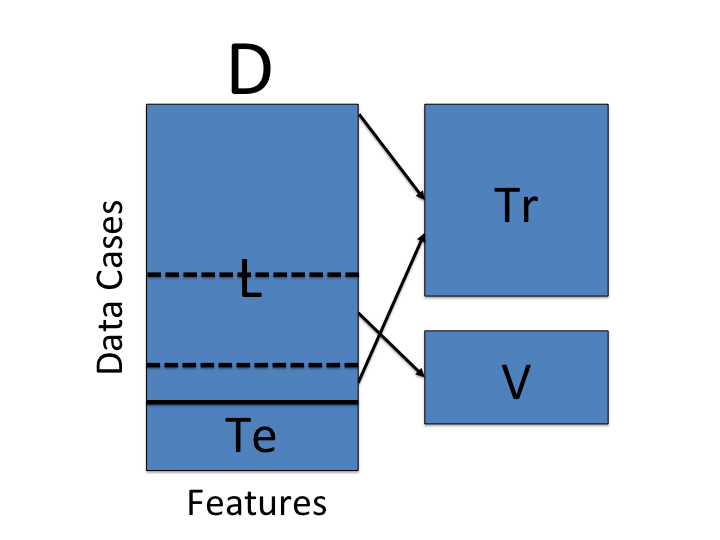
\includegraphics[width=2.8in]{../Figures/model-selection-rr-te-1.png}\\
Note that the order of the data cases needs to be randomly
shuffled before partitioning D into L and Te. 
\end{frame}

\begin{frame}[t]{Example: 3-Sample Random Resampling and Test}
\center
Second Sample\\
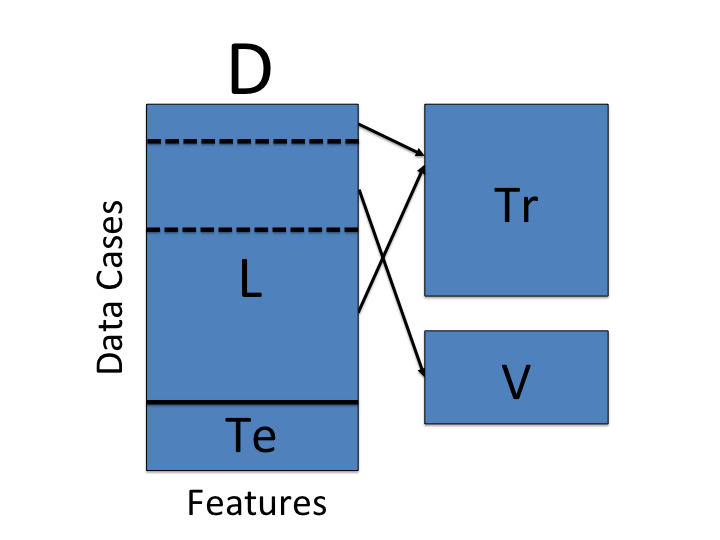
\includegraphics[width=2.8in]{../Figures/model-selection-rr-te-2.png}\\
Note that the order of the data cases needs to be randomly
shuffled before partitioning D into L and Te. 
\end{frame}

\begin{frame}[t]{Example: 3-Sample Random Resampling and Test}
\center
Third Sample\\
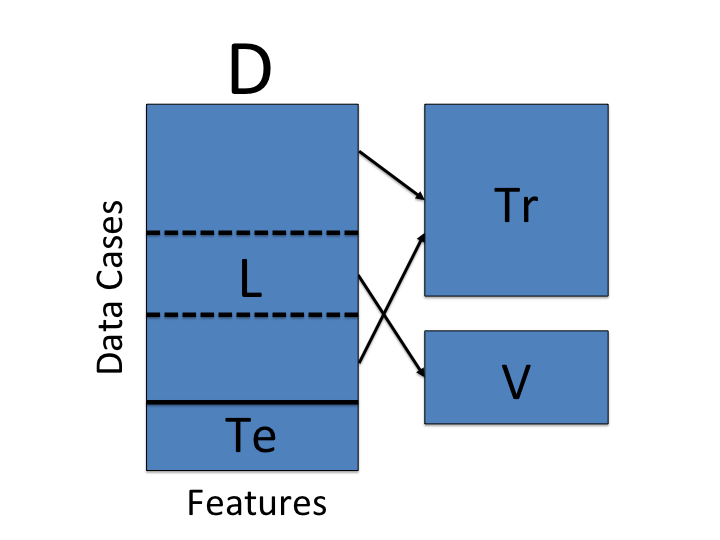
\includegraphics[width=2.8in]{../Figures/model-selection-rr-te-3.png}\\
Note that the order of the data cases needs to be randomly
shuffled before partitioning D into L and Te. 
\end{frame}



\begin{frame}[t]{Recipe 4: Crossvalidation-Crossvalidation}
\begin{itemize}
\setlength{\itemsep}{6pt}

\item Randomly partition data set $D$ into a set of $J$ blocks $C_1,...,C_J$.

\pause \item For $j=1,...,J$:
\begin{itemize}
  \pause\item Let $Te_j = C_j$ and $L_j = D/C_j$ 
  \pause\item Partition $L_j$ into a set of $K$ blocks $B_{1},...,B_{K}$.
  \pause \item For $k=1,...,K$:
  \begin{itemize}
    \pause\item Let $V=B_{k}$ and $Tr= L_j/B_k$.
    \pause\item Learn $M_{ik}$ on $Tr$ for each choice of hyperparameters $H_i$.
    \pause\item Compute error $Val_{ik}$ of $M_{ik}$ on $V$.
  \end{itemize}
  \pause\item Select hyperparameters $H_*$ minimizing $\frac{1}{K}\sum_{k=1}^K Val_{ik}$ and re-train model on $L_j$ using these hyperparameters, yielding model $M_{*j}$.
  \pause\item Compute $Err_j$ by evaluating $M_{*j}$ on $Te_j$.
\end{itemize}
\pause \item Estimate generalization error using $\frac{1}{J}\sum_{j=1}^JErr_j$

\pause \item We can define a similar nested random resampling validation procedure.

\end{itemize}

\end{frame}

\begin{frame}[t]{Trade-Offs}
\begin{itemize}
\setlength{\itemsep}{6pt}

\item In cases where the data has a benchmark split into a training set and a test set, we can use Recipes 1-3 by preserving the given test set and splitting the given training set into train and validation sets as needed.

\pause\item In cases where there is relatively little data, using a single held out test set will have high bias. In these cases, Recipe 4 often provides a better estimate of generalization error, but has much higher computational cost.

\pause\item Choosing larger $K$ in cross validation will reduce bias. Choosing larger $S$ in random re-sampling validation will reduce variance and bias. However, both increase computational costs. $K=3,5,10$ are common choices for cross validation. $K=N$, also known as Leave-one-out cross validation is also popular when feasible. 

\end{itemize}
\end{frame}



\end{document}
